\documentclass[11pt,a4paper]{article}

\usepackage[utf8]{inputenc}
\usepackage[T1]{fontenc}

\usepackage{amsmath}
\usepackage{amssymb}
\usepackage{amsthm}

\usepackage{graphicx}
\usepackage{float}

\usepackage{geometry}
\geometry{
    a4paper,
    margin=2.5cm
}

\usepackage{booktabs}
\usepackage{array}

\usepackage{xcolor}
\usepackage{listings}

\usepackage{hyperref}
\usepackage{graphicx}

\usepackage{tikz}
\usepackage{pgfplots}
\pgfplotsset{compat=1.18}

\lstset{
    basicstyle=\ttfamily\small,
    breaklines=true,
    frame=single,
    numbers=left,
    numberstyle=\tiny,
    showstringspaces=false
}

\title{
    \textbf{IX1500 Discrete Mathematics}\\
    Project 2
}

\author{
    Mo Wang\\
    \texttt{mowang@kth.se}
}

\date{September 2026}

\begin{document}

\maketitle

\begin{abstract}

This report presents the solutions to RSA encryption-decryption algorithm and problems of Project~2. The RSA algorithm includes modulus arithmetics and factorizations. The first problem considering cracking RSA is small enough to be calculated mathematically by hand by number factorization, while the second one concerns decrypting RSA problems computationally. The last one measures the execution time for both encryption and decryption, compared with different sizes of keys.

\end{abstract}

\section*{Introduction}

This report concerns implementation of an RSA encryption-decryption algorithm that uses modulus arithmetics and factorizations. 

The project consists of three parts: one hand-solved problem for a small RSA-cracking problem through small number factorization and recover the original message, while the second one concerns decrypting larger problems computationally. The third one measures the execution time for both encryption and decryption for different sizes of public exponent $e$ and private exponent $d$.

\section*{Result summary}

The result of the assignments of this project can be summarized as in Table~\ref{tab:result_summary}

\begin{table}[htbp]
\centering
\caption{Results of the three assignments in the project}
\begin{tabular}{@{}>{\bfseries}p{0.25\textwidth} p{0.65\textwidth}@{}}
\toprule
\textnormal{\textbf{Assignment number}} & \textbf{Result} \\ 
\midrule
Assignment 0 \newline (Solve by Hand) & Given RSA modulus $n=391$, public exponent $e=1$, ciphertext $c=42$, \newline Original plaintext message $m=83$ \\ \addlinespace
Assignment 1 \newline (Programming Challenge) & Message 0 is decoded using key 3 \newline (e = 29, n = 799710404000289581) \newline Message 1 is decoded using key 4 \newline (e = 29, n = 901082142384103049) \newline Message 2 is decoded using key 3 \newline (e = 29, n = 799710404000289581) \\ \addlinespace
Assignment 2 \newline (For Higher Grade) & Encryption and decryption time grows with the size of exponent, not encryption or decryption alone since both encryption and decryption is dependent on the same modular exponentation operation \\
\bottomrule
\end{tabular}

\label{tab:result_summary}
\end{table}

\section*{Assignment 0: Solve by Hand}

Given that the modulus $n$ is $n=391$, the public exponent $e$ is $e=7$ and the ciphertext $c$ is $c=42$, and consider that the private exponent is written as $d$ as well as the the decoded message as $d$, the problem can be solved by first factoring $n$, then calculating the Euler's totient function $\phi(n)$, and solve out the private exponent $d$ through $ed \equiv 1 \pmod{\phi(n)}$. Retrieving the private exponent, the original message can be simply calculated by putting it into the decryption formula $m \equiv c^d \pmod{\phi(n)}$.

\subsection*{Formula and equation}
% Add also diagrams here if possible

The number $n=391$ can be prime factored as $$n=391=17\times23$$. The Euler's totient function, $\phi(n)$ can also be calculated, since the prime factors are $17$ and $23$. This produces Euler's totient function value as $$\phi(n) = 16\times22 = 352$$.

After retreiving the Euler's totient number $\phi(n)$, the equation $$ed \equiv 1 \pmod{\phi(n)}$$ can be easily solved, by first rewriting it into a Diophantine equation, which can be further solved using GCD, Bezout's identity. Detailed steps are shown in the handwritten appendix. Finally, the private exponent $d$ turns out to be $d=151$.

With the ciphertext $c$, the private exponent $d$ and the RSA modulus $n$, the original message can be reconstructed by substituting the values into the decryption formula $m \equiv c^d \pmod{\phi(n)}$. Since the numbers are a bit large for hand-calculation, the modulus expression is decomposed into modular equation system and solved using Chinese Remainder Theorem. Detailed solution can be found in the handwritten appendix. The final result of $m$ is $m=83$.

\subsection*{Discussion}

The manual calculation of the RSA decryption algorithm shows the mathematical arithmetics behind the mechanism. The security of RSA relies on the computational difficulty asymmetry between multiplication and factorization. For a small modulus like $n = 391$, the prime factors $p=17$ and $q=23$ are trivially exposed via trial division. However, this might not be feasible for larger numbers, since a naive trial-division algorithm that tests all odd numbers or all prime numbers to the large composite number might not be efficient. Since recovering the decryption key requires computing Euler's Euler's totient function $\phi(n) = 352$ would be computationally infeasible for large keys and cannot be easily derived from RSA modulus $n$ without factorization.

The final step, evaluating $m \equiv 42^{151} \pmod{391}$, introduces a slight practical difficulty for hand calculations due to the rapidly growing exponent. Instead of naively computing the large power, modular arithmetical rules can be utilized as well as Fermat's little theorem and Chinese Remainder Theorem:
\begin{itemize}
    \item \textbf{Square-and-Multiply (Modular Exponentiation and Multiplication):} for a medium sized power, the base can be squared so that the exponent can be halved. Afterwards, modulo of base squared can be calculated, which in turns keeps the base low. The procedure can be repeated (reducing the exponent) until the exponent reaches one. $$b^{2e} = (b^2)^e \equiv B^e \pmod{n}$$ if $b \equiv B \pmod{n}$. If the exponent is odd, a factor will remain: $$b^{2e+1} = (b^2)^e \times b \equiv B^e\times b \pmod{n}$$.
    \item \textbf{Chinese Remainder Theorem (CRT):} By decomposing the large modulus $n$ into its prime moduli ($17$ and $23$), the expression can be written as several (in this case two) equations: $m_1 \equiv 42^{151} \pmod{17}$ and $m_2 \equiv 42^{151} \pmod{23}$. Applying Fermat's Little Theorem further reduces the exponents to $151 \pmod{16} = 7$ and $151 \pmod{22} = 19$, respectively. The moduli equation can be solved using Chinese Remainder Theorem.
\end{itemize}


\subsection*{Result}

The hand calculation can also be found as a screenshot in Appendix~\ref{app:handwritten}. The result is the value of the original message $$m=83$$.


\section*{Assignment 1: Programming Challenge}

The second programming task extend the RSA algorithm from the previous assignment using a larger numbers such as larger RSA moduli and public exponents, as well as given several candidate keys. Instead of manually solving the problem, a Python program with trial-division factorization implemented in C++ is used to factor the candidate RSA moduli and recover the encrypted messages in RSA to determine which key was used to encrypt each message.

The main challenge is that the messages are encrypted using one of the given RSA key, making the correct key for each message initially unknown. The problem is solved by first computing the private exponent $d$ for all the candidate keys, and applying each key to the encrypted message while manually inspect which message becomes human-readable text, in order to determine which candidate key is used.

\subsection*{Formula and equation}

For RSA, a public key consists of the modulus $n$ and public exponent $e$. If the factorization of the modulus is

\[
n = pq,
\]

where $p$ and $q$ are prime numbers, Euler's totient function can be calculated as

\[
\phi(n) = (p-1)(q-1).
\]

\subsubsection*{Factorization}

For this assignment, factorization is done by a simple and non-effective trial-and-division algorithm. A trial-and-division algorithm repeatedly trying to divide the number without any remainder with the lowest even prime number $2$ and its successive odd numbers from $3$. Whenever the number can be divided, the prime factor is added to the result prime factorization list and the process repeats until the number is indivisible by the factor.

When the number is indivisible by the current factor, the algorithm moves on to the next factor. The loop only needs to test factors fulfilling

$$ i^2 \leq n $$

because if a composite number has a factor larger than its square root, it must also have a corresponding factor smaller than its square root. If the number is not divisible by any candidates, the number is appended into the prime factors intact. The algorithm can be visualized in the listing below.

Since the code is written in C++, due to slow Python execution speed in computational-intensive loops, a bridge adapter between Python and C++ is also built using Pybind11. Additionally, a number type \texttt{uint64\_t} is also used as an unsigned 64-bit integer, since the given numbers doesn't exceed $2^{64}-1 = 1.8 \times 10^{19}$.

\begin{lstlisting}[language=C++]
std::vector<uint64_t> factorize(uint64_t n) {
    std::vector<uint64_t> factors;
    while (n % 2 == 0) {
        factors.push_back(2);
        n /= 2;
    }
    for (uint64_t i = 3; i <= n / i; i += 2) {
        while (n % i == 0) {
            factors.push_back(i);
            n /= i;
        }
    }
    if (n > 1) {
        factors.push_back(n);
    }
    return factors;
}
\end{lstlisting}

\subsubsection*{Inverse modular operation}

Once the RSA modulus can be factorized, the Euler's totient number can be also calculated, where the only step is to calculate $d$ which is the modular inverse of $e$ in $\phi(n)$:
$$ed \equiv 1 \pmod{\phi(n)}$$

This can be easily solved using extended Euclidean algorithm for solving GCD. The GCD of two numbers can be calculated by repeatedly dividing the larger number with the smaller number and assign the smaller number as the larger number and the remainder as the smaller number:

$$gcd(n, m) = gcd(m, r)$$

given that

$$n = q*m + r$$

The function \texttt{gcd\_linear\_comb} finds integers $x$ and $y$ in the equation below:

\[
xe+y\phi(n)=\gcd(e,\phi(n)).
\]

The function implements the extended Euclidean algorithm and calculates the linear combination expression.

Since a valid RSA key requires that the public exponent $e$ and the private exponent $d$ are relatively prime, in other words as the equation below:

\[
\gcd(e,\phi(n))=1,
\]

this means that a similar Diophantine equation below can be rewritten

\[
de \equiv 1 \pmod{\phi(n)}
\]
\[
de+y\phi(n)=1.
\]

where $d$ is the private exponent.

The function \texttt{gcd\_linear\_comb} is written in \texttt{util.py} where utility math functions are implemented from the ground up using only simple built-in arithmetical operations. The function computes the coefficients of a Bezout identity using the Extended Euclidean Algorithm.

The function uses itself of another utility function \texttt{gcd\_expansion} which creates the stack of linear combination. This function performs the Euclidean Algorithm and stores each division step in a stack. For every iteration, it appends the two current factors, the quotient, and the resulting remainder. The process continues until the remainder becomes zero.

\begin{lstlisting}[language=python]
def gcd_expansion(factor1: int, factor2: int) -> List[Tuple[int, int, int, int]]:
    factor_stack: List[Tuple[int, int, int, int]] = []
    while factor2 != 0:
        quotient = factor1 // factor2
        remainder = factor1 % factor2
        factor_stack.append((factor1, factor2, quotient, remainder))
        factor1 = factor2
        factor2 = remainder
    return factor_stack
\end{lstlisting}

Afterwards, the function \texttt{gcd\_linear\_comb} processes this stack in reverse order. It starts with the coefficients $x = 1$ and $y = 0$, which correspond to the last equation of the stack.

For each iteration, given that the coefficients $x$ and $y$ corresponds to the scalar bases $a$ and $b$ so that their linear combination using the scalar bases $a$ and $b$ shows $x\times a + y \times b = gcd(n, m)$. Substituting the equation with $b$ and $c$ as $c = q \times a + b$ or rewritten as $b = c - q \times a$, into $x\times a + y \times b = gcd(n, m)$ gives:
\[
\begin{aligned}
x \times a + y \times b
&= x \times a + y \times (c - q \times a) \\
&= x \times a + y \times c - y \times q \times a \\
&= y \times c + (x-y \times q) \times a
\end{aligned}
\]

Considering that the new scalar bases are $c$ and $a$, the corresponding new values of $x$ and $y$ must be: $x = y$, $y = x - y \times q$

The function \texttt{gcd\_linear\_comb} shows the algorithm implementation below.

\begin{lstlisting}[language=python]
def gcd_linear_comb(factor1: int, factor2: int) -> Tuple[int, int]:
    factor_stack: List[Tuple[int, int, int, int]] = gcd_expansion(factor1, factor2)
    x, y = 1, 0
    for factor1, factor2, quotient, remainder in reversed(factor_stack):
        x, y = y, x - quotient * y
    return x, y
\end{lstlisting}

\subsubsection*{Power modulus}

For modular exponentiation, the program uses the \texttt{power\_modulo} function. The function implements the square-and-multiply method rather than computing the large $c^d$ directly and then apply the modulo operator. For calculating $c^d \mod n$, the algorithm first calculates the modulus of $c$:
$$c^d \equiv e^d \pmod{n} $$
if $c \equiv e \pmod{n}$.

Afterwards, if the exponent $d=2m+1$ is odd, then it can be reduced as

Afterwards, if the exponent $d=2m+1$ is odd, the expression can be rewritten as:
$$c^d = c^(2m+1) = (c^m)^2*c$$

Otherwise, if the exponent $d=2m$ is even, the expression can be instead rewritten as:
$$c^d = c^(2m) = (c^m)^2$$

If a factor $c$ appears, it will be multiplied into a separate accumulator \texttt{result} and taking the modulus operator with the given modulo. The rest $$(c^m)^2$$ will be processed as the even case. In this case, the base $c^m$ can be reduced by taking the modulo operator.

The listing below shows the operation of a power modulus. The odd-even parity is checked using the boolean AND operator with \texttt{0b1}, since only odd numbers has the least significant bit as 1. Additionally, a right shift by one step is also equivalent for an integer division by 2. Despite Python may not make an shifting operator cheaper than an integer division, as in C/C++, the reason of the indirection is due to programming habits.

\begin{lstlisting}[language=python]
def power_modulo(base: int, exponent: int, modulo: int) -> int:
    result = 1
    base = base % modulo
    while exponent > 0:
        if exponent & 1: # if number is odd
            result = (result * base) % modulo
        base = (base * base) % modulo
        exponent >>= 1 # exponent = exponent / 2
    return result
\end{lstlisting}

Once $d$ has been calculated, each ciphertext value $c$ can be decrypted according to

\[
m \equiv c^d \pmod n.
\]

The program then applies the decryption formula to every ciphertext in \texttt{messages} using both candidate private keys.

\subsection*{Discussion}

The assignment 1 relies on converting the manual implementation steps into code. This is especially useful in terms of calculation of modular exponentiation which may involve an extremely large intermediate integer $c^d$. However, the difference between Assignment 0 and Assignment 1 is that arithmetical operations for larger numbers, if not too big, does not need to be aggressively simplified, since processors are handling 32-bit integers comfortly. This means that modular exponentiation may not always require Fermat's little theorem and Euler's theorem without degrading algorithm performance.

The factorization of the RSA modulus is the most computationally heavy bottleneck of the program. The reason is that the public key contains $n$ and $e$, but the private exponent $d$ requires $\phi(n)$ which cannot be derived from any given numbers without factoring the number $n$. The implemented factorization algorithm is a simple trial-division algorithm, which is sufficient for the modulus used in this assignment. But for larger number than given in this assignment, the execution time degrades with the growing size of the number to be factorized.

After calculating the private exponent for each candidate key, the program decrypts every message with that key. This produces several candidate plaintexts, which most of them do not form any meaningful text at all. A function \texttt{is\_text} is used to check if the text is readable, by checking if all of the message string contains common letters, numbers or useful symbols. 

\subsection*{Result}

The results of the keys for each of the three messages are summarized in Table~\ref{tab:assignment1-results}. As a result, Messages 0 and 2 were encrypted using the first RSA modulus, while Message 1 was encrypted using the second modulus.

\begin{table}[H]
\centering
\caption{Results from the RSA programming challenge}
\label{tab:assignment1-results}
\begin{tabular}{@{}c c c c@{}}
\toprule
\textbf{Message} & \textbf{Key} & \textbf{$e$} & \textbf{$n$} \\
\midrule
Message 0 & Key 3 & 29 & 799710404000289581 \\
Message 1 & Key 4 & 29 & 901082142384103049 \\
Message 2 & Key 3 & 29 & 799710404000289581 \\
\bottomrule
\end{tabular}
\end{table}

\section*{Assignment 2: For Higher Grade}

The last assignment is to implement the RSA cryptography system and investigation of the execution time and computational costs. This is divided into two parts, where the first is the impact of public exponent number size (in bits) of the execution time with fixed public exponent, and the second is the impact of RSA modulus on execution time while fixing private exponent.

\subsection*{Formula and equation}

In terms of implementation of a RSA cryptography that encrypts and decrypts different messages, a pair of public and private keys are built. The RSA uses a public key $(n, e)$ and a private key $(n, d)$. The modulus can be constructed by choosing two prime numbers $p$ and $q$ such that:

$$ n = pq $$

whereas the Euler's totient function of the modulus can be calculated as:

$$ \phi(n) = (p-1)(q-1) $$

After calculating these, the public exponent $e$ is selected so that the public exponent $e$ and the RSA modulus $\phi(n)$ are relatively prime to each other:

$$ \gcd(e,\phi(n))=1 $$

A simple solution of generating a prime number as a public exponent, since a prime number and other arbitrary number are always relatively prime to each other.

After generating the key pairs (public and private keys), encryption and decryption can be taken place. For a plaintext block $m$, RSA encryption can be performed as

$$ c \equiv m^e \pmod n $$

where $c$ is the resulting ciphertext block. Decryption is performed using

$$
m \equiv c^d \pmod n.
$$

In order to encrypt and decrypt plaintext messages from ASCII strings, they must be converted into numeral blocks, which are implemented in \texttt{enc\_util.py} and does not have dependencies. Since an ASCII character is 8 bits, which means it can take $2^8 = 256$ different values. Given an RSA modulus $n$, a numeral block can encode at most $m = \lfloor log_{256}(n) \rfloor$ character using \texttt{encode\_message}. The remaining ASCII characters that doesn't fit perfectly into $m$ bytes are also encoded while padding the missing bytes with 0, since a null byte with value zero marks the end of a string anyway. By using this, numbers can be converted into large numbers, where RSA encryption and decryption mechanism can be applied. Decryption mechanism works in the reversed where the number is decoded into a number of ASCII characters. 

The decrypted blocks are then converted back into characters. As a correctness check, the recovered plaintext is compared afterwards with the original message.

$$
\text{recovered message}=\text{original message}.
$$

\subsection*{2.1 RSA computational cost}

The first computational cost analysis investigates how the size of the RSA modulus affects computational cost. Three RSA key sizes are tested with predefined 32, 64, and 128 bits numbers for both prime numbers, while the public exponent is kept fixed at $e=65537$, which is a large prime number.

Each encryption and decryption operation is repeated 300 times, timed using \texttt{time.perf\_counter()}. Afterwards, the encryption and decryption times are then divided by the number of plaintext blocks to calculate an average time per block.

The measured results can be shown as the table below in Table~\ref{tab:key-scale}:

\begin{table}[ht]
    \centering
    \caption{Effect of RSA key size on encryption and decryption time.}
    \label{tab:key-scale}
    \begin{tabular}{lrrrrr}
        \toprule
        Size & Bits of $n$ & Blocks &
        $T_{\mathrm{enc}}$ ($\mu$s/block) &
        $T_{\mathrm{dec}}$ ($\mu$s/block) &
        Bits of $d$ \\
        \midrule
        Small  & 32  & 54 & 2.60 & 5.66  & 31  \\
        Medium & 64  & 24 & 3.30 & 15.55 & 62  \\
        Large  & 128 & 11 & 3.80 & 41.77 & 127 \\
        \bottomrule
    \end{tabular}
\end{table}

Additionally, the measured results can also be visualized clearly as a line graph in Figure~\ref{fig:key-scale-time}.

\begin{figure}[ht]
    \centering
    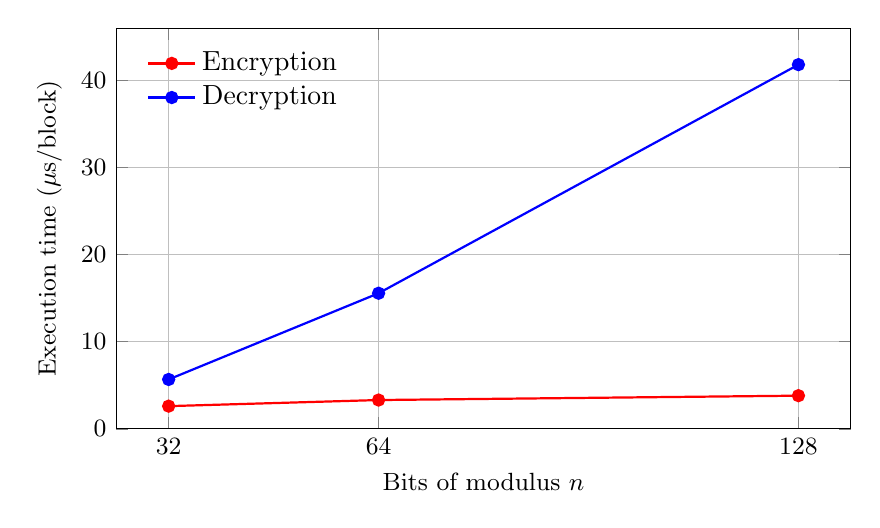
\begin{tikzpicture}
        \begin{axis}[
            width=0.9\textwidth,
            height=0.55\textwidth,
            xlabel={Bits of modulus $n$},
            ylabel={Execution time ($\mu$s/block)},
            xmin=24,
            xmax=136,
            ymin=0,
            grid=major,
            legend pos=north west,
            legend style={
                draw=none,
                fill=none
            },
            tick label style={font=\small},
            label style={font=\small},
            xtick={32,64,128},
        ]

        % Encryption
        \addplot[
            red,
            thick,
            mark=*,
            mark size=2pt
        ] coordinates {
            (32,2.60)
            (64,3.30)
            (128,3.80)
        };
        \addlegendentry{Encryption}

        % Decryption
        \addplot[
            blue,
            thick,
            mark=*,
            mark size=2pt
        ] coordinates {
            (32,5.66)
            (64,15.55)
            (128,41.77)
        };
        \addlegendentry{Decryption}

        \end{axis}
    \end{tikzpicture}

    \caption{Effect of RSA key size on encryption and decryption time.}
    \label{fig:key-scale-time}
\end{figure}

Both encryption and decryption becomes more expensive as the modulus increases in size. According to the table, encryption increases from approximately $2.60 \mu$s each block for the 32-bit modulus to $3.80 \mu$s per block for the 128-bit modulus. For decryption, the increase is substantially larger, where the decryption time increases from $5.66 \mu$s per block for 32 bits to $41.77 \mu$s per block for 128 bits.

The reason is that both exponents and modulus number contributes to the execution time. Since both encryption and decryption involves modular exponentiation, neither encryption nor decryption can generally be considered as fastest or slowest for any number. In this benchmark setup, the public exponent is fixed to $65537$, with only 17 bits. However, the private exponent is allowed to grow and has sizes 31, 62 and 127 bits. A larger exponent contributes directly to longer execution time for modular exponential algorithm, since the exponent is halved for each iteration and has a logarithmic growth to the exponent.

A larger modulo can also affect execution time, but not directly. Since \texttt{int} in Python is essentially a big integer, meaning that it can stretch into any size, arithmetic operations for large numbers can take longer execution time.

% The reduction in the number of plaintext blocks as the modulus grows is a consequence of the larger block size. The 128-bit modulus can contain more characters in each plaintext block than the 32-bit modulus.

\subsection*{2.2 Effect of RSA exponents on encryption and decryption time}

In the second computational cost analysis, the RSA modulus is fixed at a 128-bit integer number $n = 185879242930562613603547896228926251273$, which can be prime factorized into two 64-bit numbers $17524406870024073221$ and $10606877842382991413$. The two numbers are obtained through fast generation of large prime numbers using \texttt{SymPy}, and the numbers are multiplied afterwards. These are two randomly generated after executing the script below:

\begin{lstlisting}[language=python]
def generate_prime(bits: int = 64) -> int:
    lower = 1 << (bits - 1)
    upper = (1 << bits) - 1

    while True:
        candidate = random.randrange(lower, upper) | 1

        if isprime(candidate):
            return candidate
\end{lstlisting}

Several valid values of the public exponent $e$ is tested (all prime numbers):

$$ 3,\quad17,\quad257,\quad65537,\quad16777259, \quad1099511627791 $$

These are predefined prime numbers for 2 bits, 5 bits, 9 bits, 17 bits, 25 bits respectively 41 bits. Since a prime number and another arbitrary number that is different from the chosen number is relatively prime, the private exponent $d$ can be safely calculated and guarenteed to be always existing. For each value of $e$, the corresponding private exponent $d$ can be calculated from

$$
ed \equiv \pmod{\varphi(n)}.
$$

Scaling the public exponent $e$, the results can be shown in the Table~\ref{tab:public-exponent-scale}:

\begin{table}[ht]
    \centering
    \caption{Effect of public exponent size on RSA encryption and decryption time.}
    \label{tab:public-exponent-scale}
    \begin{tabular}{rrrrr}
        \toprule
        $e$ & Bits of $e$ & Bits of $d$ &
        $T_{\mathrm{enc}}$ (ms) & $T_{\mathrm{dec}}$ (ms) \\
        \midrule
        3             & 2  & 127 & 0.007 & 0.484 \\
        17            & 5  & 127 & 0.014 & 0.536 \\
        257           & 9  & 127 & 0.024 & 0.473 \\
        65537         & 17 & 127 & 0.047 & 0.500 \\
        16777259      & 25 & 127 & 0.077 & 0.814 \\
        1099511627791 & 41 & 128 & 0.218 & 0.807 \\
        \bottomrule
    \end{tabular}
\end{table}

The scaling behavior can also be clearly visualized in the Figure~\ref{fig:public-exponent-time} below as well:
\begin{figure}[ht]
    \centering
    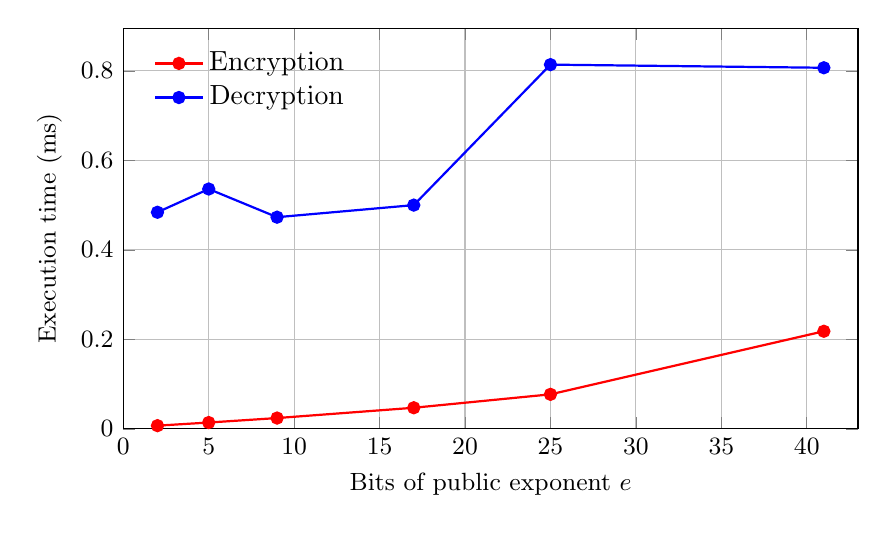
\begin{tikzpicture}
        \begin{axis}[
            width=0.9\textwidth,
            height=0.55\textwidth,
            xlabel={Bits of public exponent $e$},
            ylabel={Execution time (ms)},
            xmin=0,
            xmax=43,
            ymin=0,
            grid=major,
            legend pos=north west,
            legend style={
                draw=none,
                fill=none
            },
            tick label style={font=\small},
            label style={font=\small},
        ]

        % Encryption
        \addplot[
            red,
            thick,
            mark=*,
            mark size=2pt
        ] coordinates {
            (2,0.007)
            (5,0.014)
            (9,0.024)
            (17,0.047)
            (25,0.077)
            (41,0.218)
        };
        \addlegendentry{Encryption}

        % Decryption
        \addplot[
            blue,
            thick,
            mark=*,
            mark size=2pt
        ] coordinates {
            (2,0.484)
            (5,0.536)
            (9,0.473)
            (17,0.500)
            (25,0.814)
            (41,0.807)
        };
        \addlegendentry{Decryption}

        \end{axis}
    \end{tikzpicture}

    \caption{Effect of public exponent size on RSA encryption and decryption time.}
    \label{fig:public-exponent-time}
\end{figure}


The encryption time generally increases as the size of $e$ increases. It increases from $0.007$ ms for the 2-bit exponent $e=3$ to $0.218$ ms for the 41-bit exponent.

The reason can be found in repeated-squaring implementation of the \texttt{power\_modulo} for modular exponentiation. A larger exponent requires more iteration, in the same way as described for scaling different bits of keys.

However, the decryption time does not show similar relationship when $e$ is scaled. This is because decryption uses $d$, rather than $e$. In the benchmark, the private exponent has approximately 127--128 bits for all tested values of $e$, which makes the decryption times similar throughout the growth of exponent $e$.

Another benchmark is also performed by scaling the private exponent $d$, using the same number set as the previous benchmark for $e$. In this case, the public exponent $e$ is derived from $d$ using modular inverse.

The results can be shown in the Table~\ref{tab:private-exponent-scale} below:

\begin{table}[ht]
    \centering
    \caption{Effect of private exponent size on RSA encryption and decryption time.}
    \label{tab:private-exponent-scale}
    \begin{tabular}{rrrrr}
        \toprule
        $d$ & Bits of $d$ & Bits of $e$ &
        $T_{\mathrm{enc}}$ (ms) & $T_{\mathrm{dec}}$ (ms) \\
        \midrule
        3             & 2  & 127 & 0.790 & 0.009 \\
        17            & 5  & 127 & 0.535 & 0.015 \\
        257           & 9  & 127 & 0.532 & 0.043 \\
        65537         & 17 & 127 & 0.478 & 0.045 \\
        16777259      & 25 & 127 & 0.493 & 0.071 \\
        1099511627791 & 41 & 128 & 0.547 & 0.117 \\
        \bottomrule
    \end{tabular}
\end{table}

The same dataset can also be visualized below cleanly as a line graph in Figure~\ref{fig:private-exponent-time}

\begin{figure}[ht]
    \centering
    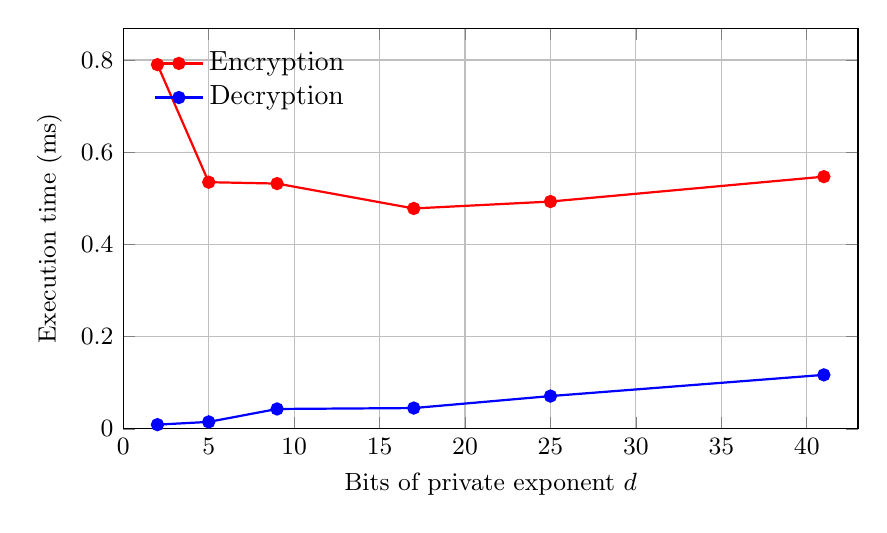
\begin{tikzpicture}
        \begin{axis}[
            width=0.9\textwidth,
            height=0.55\textwidth,
            xlabel={Bits of private exponent $d$},
            ylabel={Execution time (ms)},
            xmin=0,
            xmax=43,
            ymin=0,
            grid=major,
            legend pos=north west,
            legend style={
                draw=none,
                fill=none
            },
            tick label style={font=\small},
            label style={font=\small},
        ]

        % Encryption
        \addplot[
            red,
            thick,
            mark=*,
            mark size=2pt
        ] coordinates {
            (2,0.790)
            (5,0.535)
            (9,0.532)
            (17,0.478)
            (25,0.493)
            (41,0.547)
        };
        \addlegendentry{Encryption}

        % Decryption
        \addplot[
            blue,
            thick,
            mark=*,
            mark size=2pt
        ] coordinates {
            (2,0.009)
            (5,0.015)
            (9,0.043)
            (17,0.045)
            (25,0.071)
            (41,0.117)
        };
        \addlegendentry{Decryption}

    \end{axis}
    \end{tikzpicture}

    \caption{Effect of private exponent size on RSA encryption and decryption time.}
    \label{fig:private-exponent-time}
\end{figure}

From these results, the reversed effect can be observed. Since decryption uses $d$, the decryption time generally increases as the integer size of $d$ incrases. This can be shown that the measured time increases from $0.009$ ms for the 2-bit value $d=3$ to $0.117$ ms for the 41-bit value.

On the other hand, the encryption time flunctuates around at some constant value since corresponding public exponents have around 127 to 128 bits as well. 

\subsection*{Discussion}

The benchmark analysis above shows that the RSA computational cost is strongly connected to the size of the exponent in modular exponentation. Additionally, the cost has some relationship with the RSA modulus. The reason is that the modular exponentation implements square-and-multiply method, where as the number of square operations grows logarithmically with the exponent number. However, a large modulus number can also slightly slow down the modulo operator execution as well.

The first benchmark shows that increasing the modulus size increases both encryption and decryption cost, where the effect for decryption is particularly visible since the private exponent is fixed as $e=65537$. The second experiment provides a more direct demonstration of the influence of the exponent. When $e$ is increased while $n$ remains fixed, the encryption time generally increases. The measured encryption time increases from $0.007$ ms for a 2-bit exponent to $0.218$ ms for a 41-bit exponent.

Additionally, since fluctuation in measured benchmark happens, the exponent size gives only a useful hint of the computational cost and its growth trend, but it doesn't determine the exact execution time or cost.

\subsection*{Result}

Using the RSA implementation with benchmarks, the computational measurements can be shown as below:

\begin{itemize}
\item Increasing the RSA modulus increases both encryption and decryption time.
\item Decryption is substantially slower than encryption for the tested 128-bit key with $e=65537$.
\item Increasing the public exponent generally increases encryption time.
\item Increasing the private exponent generally increases decryption time.
\item Exponent size in bits and execution time are related, but the relationship is not perfectly a linear relationship.
\end{itemize}

The graphs corresponding to these measurements show the same trends visually. The first pair of graphs shows encryption and decryption time as a function of RSA key size. The second pair shows the effect of changing the public/private exponent size while keeping the modulus fixed.

\section*{Program structure}

The program structure consists of multiple program files, grouped by category below:
\begin{lstlisting}
- Assignment high-level files:
  - assignment1_consts.py
  - assignment1.py
  - assignment2_consts.py
  - assignment2.py
  
- Python utility files:
  - enc_util.py
  - util.py
  
- C++ factorization using pybind11:
  - factor_wrap.cpp
  - factor.cpp
  - factor.py
  - Makefile
  
- Probe file:
  - gen_large_prime.py
\end{lstlisting}
The following files are found separately as submission.

The program files \texttt{util.py} and \texttt{enc\_util.py} are Python utility modules that contain common arithmetic operations, such as modular exponentiation and the conversion of ASCII strings into numerical blocks for RSA computations. These functions are essentially simple RSA-arithmetical building blocks for the assignment programs and do not rely on external dependencies except Python's static typing functionality  \texttt{typing} and the \texttt{time} module for benchmarking. The utility functions are built from the ground up using Python's built-in operators.

Additionally, the program file \texttt{factor.cpp} contains trial-division algorithm for integer factorization implemented in C++ that can handle computational intensive loops faster. The file \texttt{factor\_wrap.cpp} provides a C++-side \texttt{pybind11} wrapper, which can be invoked from the Python stub file \texttt{factor.py}. However, in order to import \texttt{factor.py}, both C++ files must be compiled into a shared object file, which can be done by running \texttt{make} using the file \texttt{Makefile}. The compilation is platform-dependent and guaranteed to be working on Linux Ubuntu 22.04 or WSL with Linux Ubuntu 22.04. Both GNU toolchain \texttt{g++} for C++ and \texttt{pybind11} for Python invocation is required in order to compile respectively invoke the shared object file from Python. \texttt{pybind11} can be installed using \texttt{pip install -r pybind11>=2.10}.

Finally, the files \texttt{assignment1.py} and \texttt{assignment2.py} contain high-level implementation of the assignments depending on the mentioned utility functions. the files \texttt{assignment1\_consts.py} and \texttt{assignment2\_consts.py} contain the necessary constant values needed for computing results of assignments, such as RSA keys and encrypted messages. The reason for the separation is to avoid unnecessary data from cluttering the implementation files.

Lastly, the file \texttt{gen\_large\_prime.py} is used only to generate and obtain two random 64-bit unsigned integer primes for task 2.2. It is not used as utility function to any library.

\begin{thebibliography}{9}

\bibitem{boiers}
Lars-Christer Böiers,
\textit{Diskret matematik},
2nd ed.,
Studentlitteratur AB, 2003.
ISBN: 9789144031026.

\bibitem{lectures}
IX1500 Discrete Mathematics, lecture notes F10--F12.

\end{thebibliography}

\clearpage
\appendix

\section{Handwritten solution for assignment 0}
\label{app:handwritten}

\begin{figure}[htbp]
    \centering
    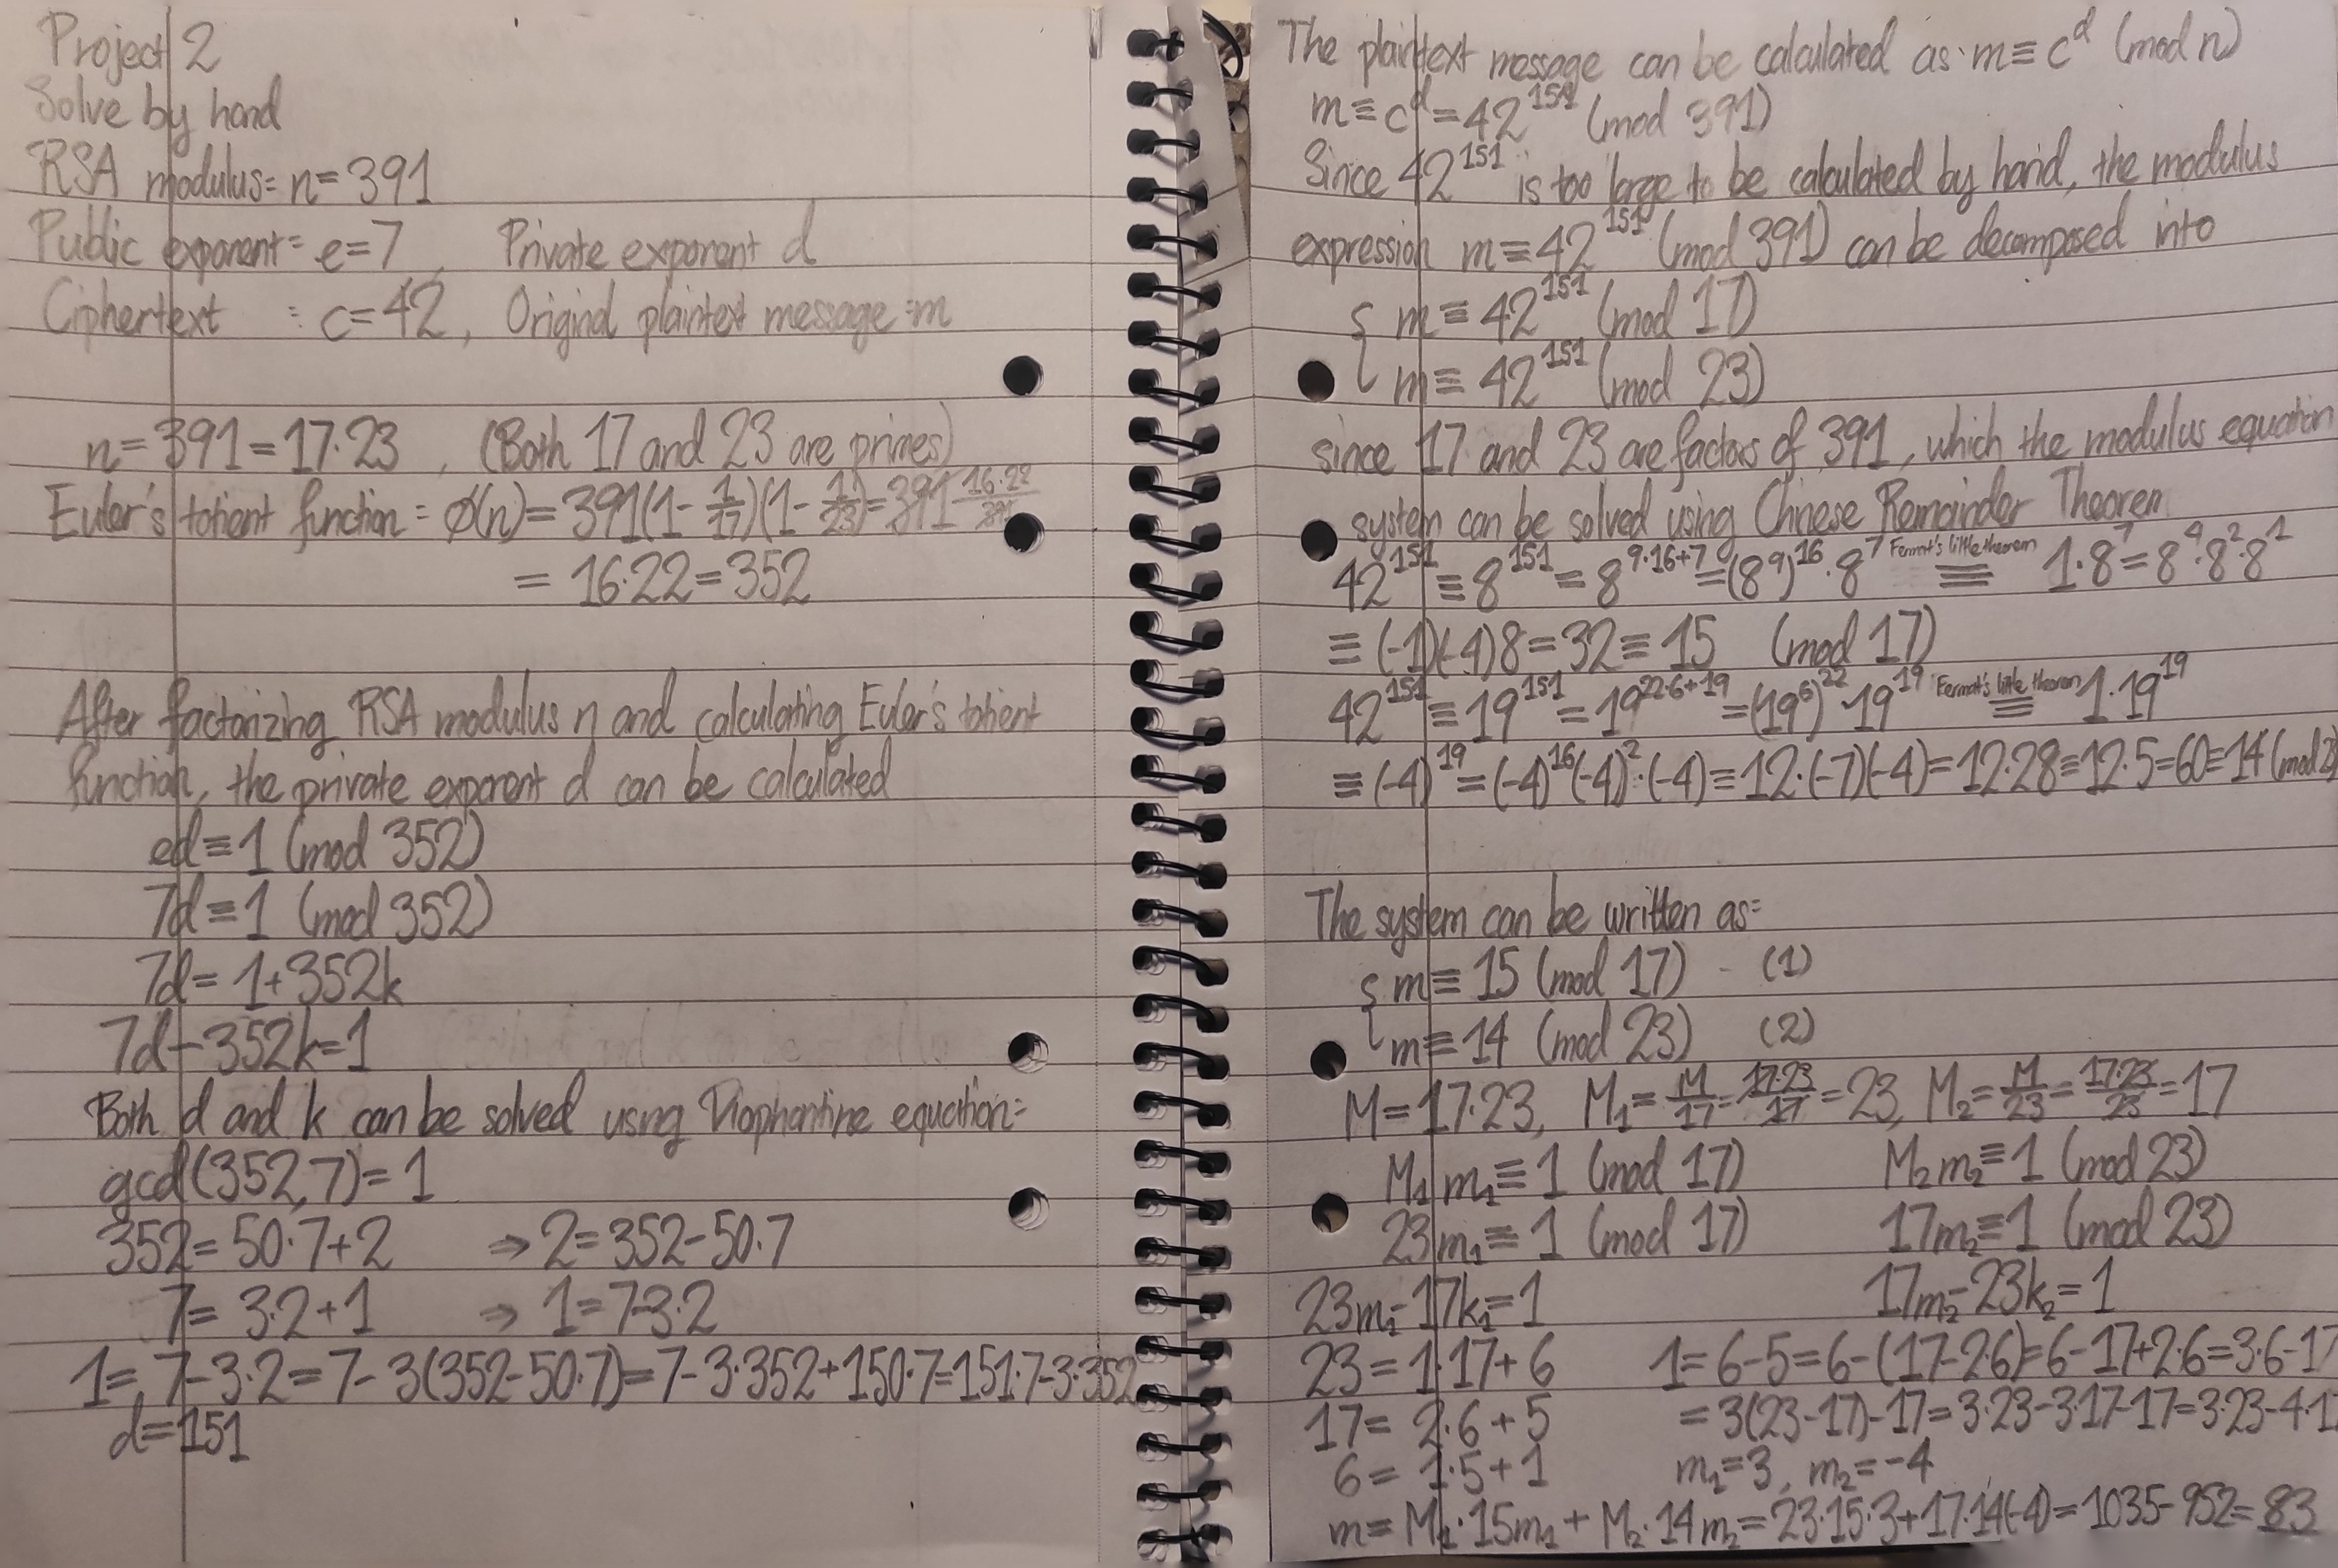
\includegraphics[width=\textwidth]{handwritten_2.jpg}
    \caption{Screenshot of the application.}
    \label{fig:screenshot}
\end{figure}

\end{document}